\documentclass{article} % For LaTeX2e
\usepackage{nips15submit_e,times}
\usepackage{hyperref}
\usepackage{url}
\usepackage{natbib}
%\documentstyle[nips14submit_09,times,art10]{article} % For LaTeX 2.09
\usepackage{amsthm}
\usepackage{amsmath}
\usepackage{amssymb}
\usepackage{graphicx}
\usepackage{epstopdf}
\usepackage{array}
\usepackage{xspace}
\usepackage{enumerate}
\usepackage{paralist}
\usepackage[capitalize]{cleveref}

% For algorithms
\usepackage{algorithm}
\usepackage{algorithmic}

\title{Easy Data for Independent Component Analysis}


\author{
Ruitong Huang \\
Department of Computing Science\\
University of Alberta \\
Edmonton, AB T6G2E8 Canada\\
\texttt{ruitong@ualberta.ca} \\
\And
Andr\'as Gy\"orgy \\
Department of Electrical and Electronic Engineering\\ 
Imperial College London\\ 
South Kensington Campus, London SW7 2BT, UK \\
\texttt{a.gyorgy@imperial.ac.uk} \\
\And
Csaba Szepesv\'ari \\
Department of Computing Science\\
University of Alberta \\
Edmonton, AB T6G2E8 Canada\\
\texttt{szepesva@ualberta.ca}
}

% The \author macro works with any number of authors. There are two commands
% used to separate the names and addresses of multiple authors: \And and \AND.
%
% Using \And between authors leaves it to \LaTeX{} to determine where to break
% the lines. Using \AND forces a linebreak at that point. So, if \LaTeX{}
% puts 3 of 4 authors names on the first line, and the last on the second
% line, try using \AND instead of \And before the third author name.

\newcommand{\norm}[1]{\|#1\|}
\newcommand{\fix}{\marginpar{FIX}}
\newcommand{\new}{\marginpar{NEW}}
\newcommand{\iid}{i.i.d.\xspace}
\newcommand{\ra}{\rightarrow}
\newcommand{\real}{\mathbb{R}}
\renewcommand{\natural}{\mathbb{N}}
\DeclareMathOperator{\pol}{Poly}
\newcommand{\poly}[1]{\pol\left(#1\right)}
\newcommand{\E}{\mathbb{E}}
\newcommand{\eps}{\epsilon}
\renewcommand{\epsilon}{\varepsilon}

\newtheorem{lemma}{Lemma}[section]
\newtheorem{thm}[lemma]{Theorem}
\newtheorem{claim}[lemma]{Claim}
\newtheorem{cor}[lemma]{Corollary}
\newtheorem{example}[lemma]{Example}
\newtheorem{prop}[lemma]{Proposition}
\theoremstyle{definition}
\newtheorem{definition}[lemma]{Definition}
\newtheorem{remark}[lemma]{Remark}
\newtheorem*{solution}{Solution}
\newtheorem{note}[lemma]{Note}
\newtheorem{problem}[lemma]{Problem}
\newtheorem{assumption}[lemma]{Assumption}
\nipsfinalcopy % Uncomment for camera-ready version

\begin{document}


\maketitle

\begin{abstract}
We study independent component analysis with noisy observations in a deterministic framework. We present a consistent, polynomial-time algorithm to reconstruct the mixing matrix with a data-dependent error bound. In contrast to earlier work, our results hold without any stochastic assumptions on the source signals and the observation noise. When applied
to the standard i.i.d.\ stochastic ICA model, 
our algorithm, for the first time in the literature, achieves a reconstruction error that vanishes at a $1/\sqrt{T}$ rate using $T$ observations and scales only polynomially with the natural parameters of the problem.  
\end{abstract}

\section{Introduction}
Independent Component Analysis (ICA) is a data analysis technique that attempts to explain an observed $x\in \real^{d\times T}$ array by decomposing it into the product $A s$ where $A\in \real^{d\times d}$ is a non-singular matrix and $s\in \real^{d\times T}$ is viewed as $T$ $d$-dimensional vector such that the components of the vectors are ``statistically independent'' \citep{HyKaOj01}.
Oftentimes, this is illustrated by data as shown in \cref{fig:demo}. 
On the left-hand side of this figure, the bottom three plots depict the $d=3$ components of the observed signal $x$. 
The $x$ axis represents time: The numbers shown are scaled by a factor of $500$; thus $T=2500$.
This observed data $x$ is generated by mixing the sources shown by the top three graphs on the left-hand side. 
Reconstruction results by three algorithms are shown on the right-hand side. As can be seen, 
up to scaling and the ordering of the reconstructed components, the reconstruction is quite successful no matter the algorithms.
The curious thing about this example is that the all components of the source data are periodic functions of time. This is quite obvious for the first two components, while the third, being generated using a pseudo-random number generator has a long period and thus ``looks random''.
Are the components $s_1(t)$ and $s_2(t)$ (or $s_1(t)$ and $s_3(t)$) independent of each other 
as required by the standard ICA modelling assumptions? Of course they are!
As the reader may recall,
any two numbers $a,b\in \real$ when viewed as random variables, i.e., constant functions from an underlying probability space,
are independent of each other, hence $s_1(t)$ and $s_2(t)$ will be independent, as will be $s_1(t)$ and $s_3(t)$, or 
even $s_1(t)$ and $(s_2(t),s_3(t))$.
Does the success of the algorithms on this example imply 
	that they will also work when used on the mixture of \emph{any} source? 
Of course not. For example, if one source is a linear function of another source then no algorithm can recover the sources from their mixtures. Another question is whether the temporal dependency of the sources may hamper performance. If $s(1) = s(2) = \dots = s(T)$ then the algorithms effectively need to work with a single vector observation and no algorithm will be able to perform a successful reconstruction. Some data is (as shown) is easy, some will be harder if not impossible to work.
What makes then some data easy (or hard) to work with when it comes to independent component analysis?
Can we redefine the problem of ICA in a meaningful way so that we can explain the success of the particular ICA algorithms on the above example?

In this short communication we give a summary of our longer paper \citep{HuGySze15} where we attempted to provide some answers to these questions, while we also streamline the presentation of the results. 
At a high level, the essence of our approach is to define empirical measures of the ``niceness'' of data 
and a measure of the success of the algorithm and then postulating the requirement that good algorithm are those that get better results on ``nicer'' data. We also require that the niceness measure should behave in a controlled fashion in the classical
ICA settings so that the usual statistical results can be recovered from our results.
The key feature of the approach is that no probabilistic assumptions are made on the data (the algorithms may randomize though), and thus this work can be thought as the natural extension of online learning
where learning algorithms are analyzed without making any probabilistic assumptions \citep{CBLu06:book}.
\begin{figure}[h]
\centering
	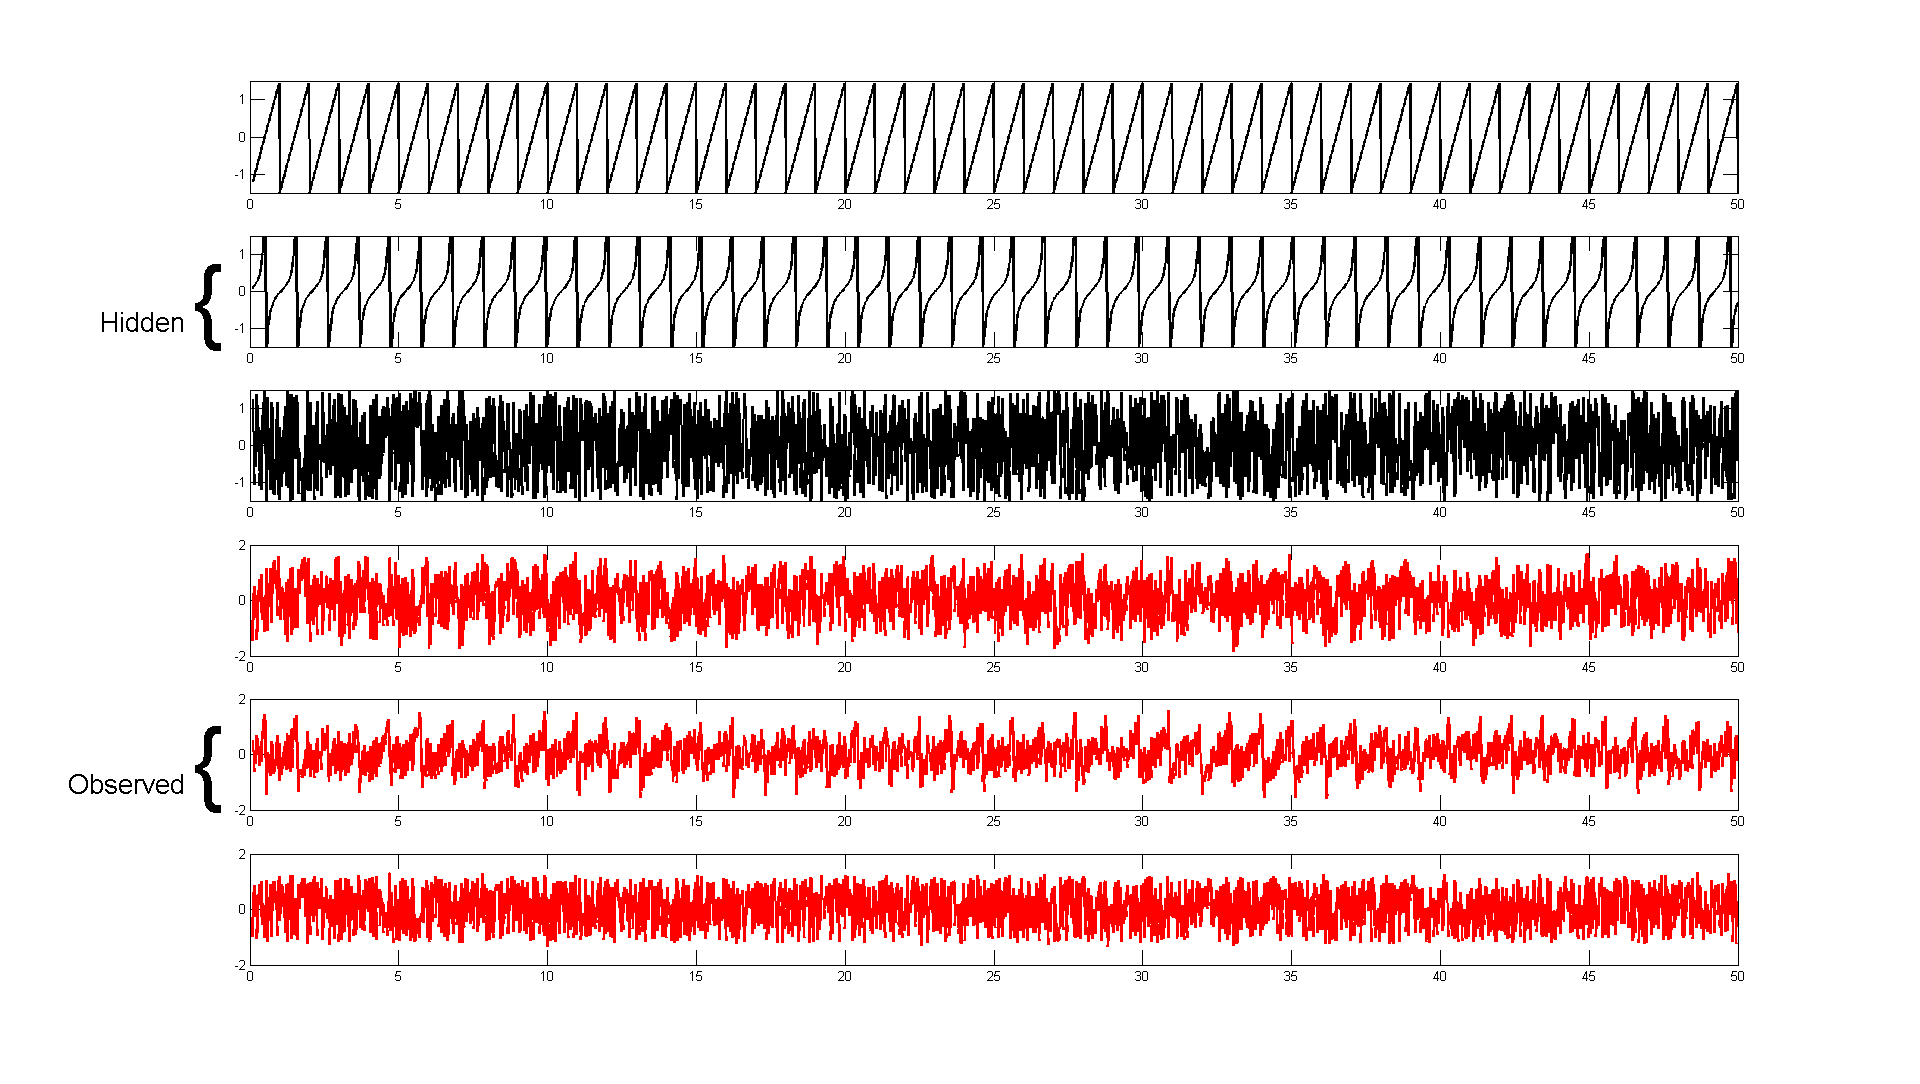
\includegraphics[width = 0.49\linewidth]{demo_source}
	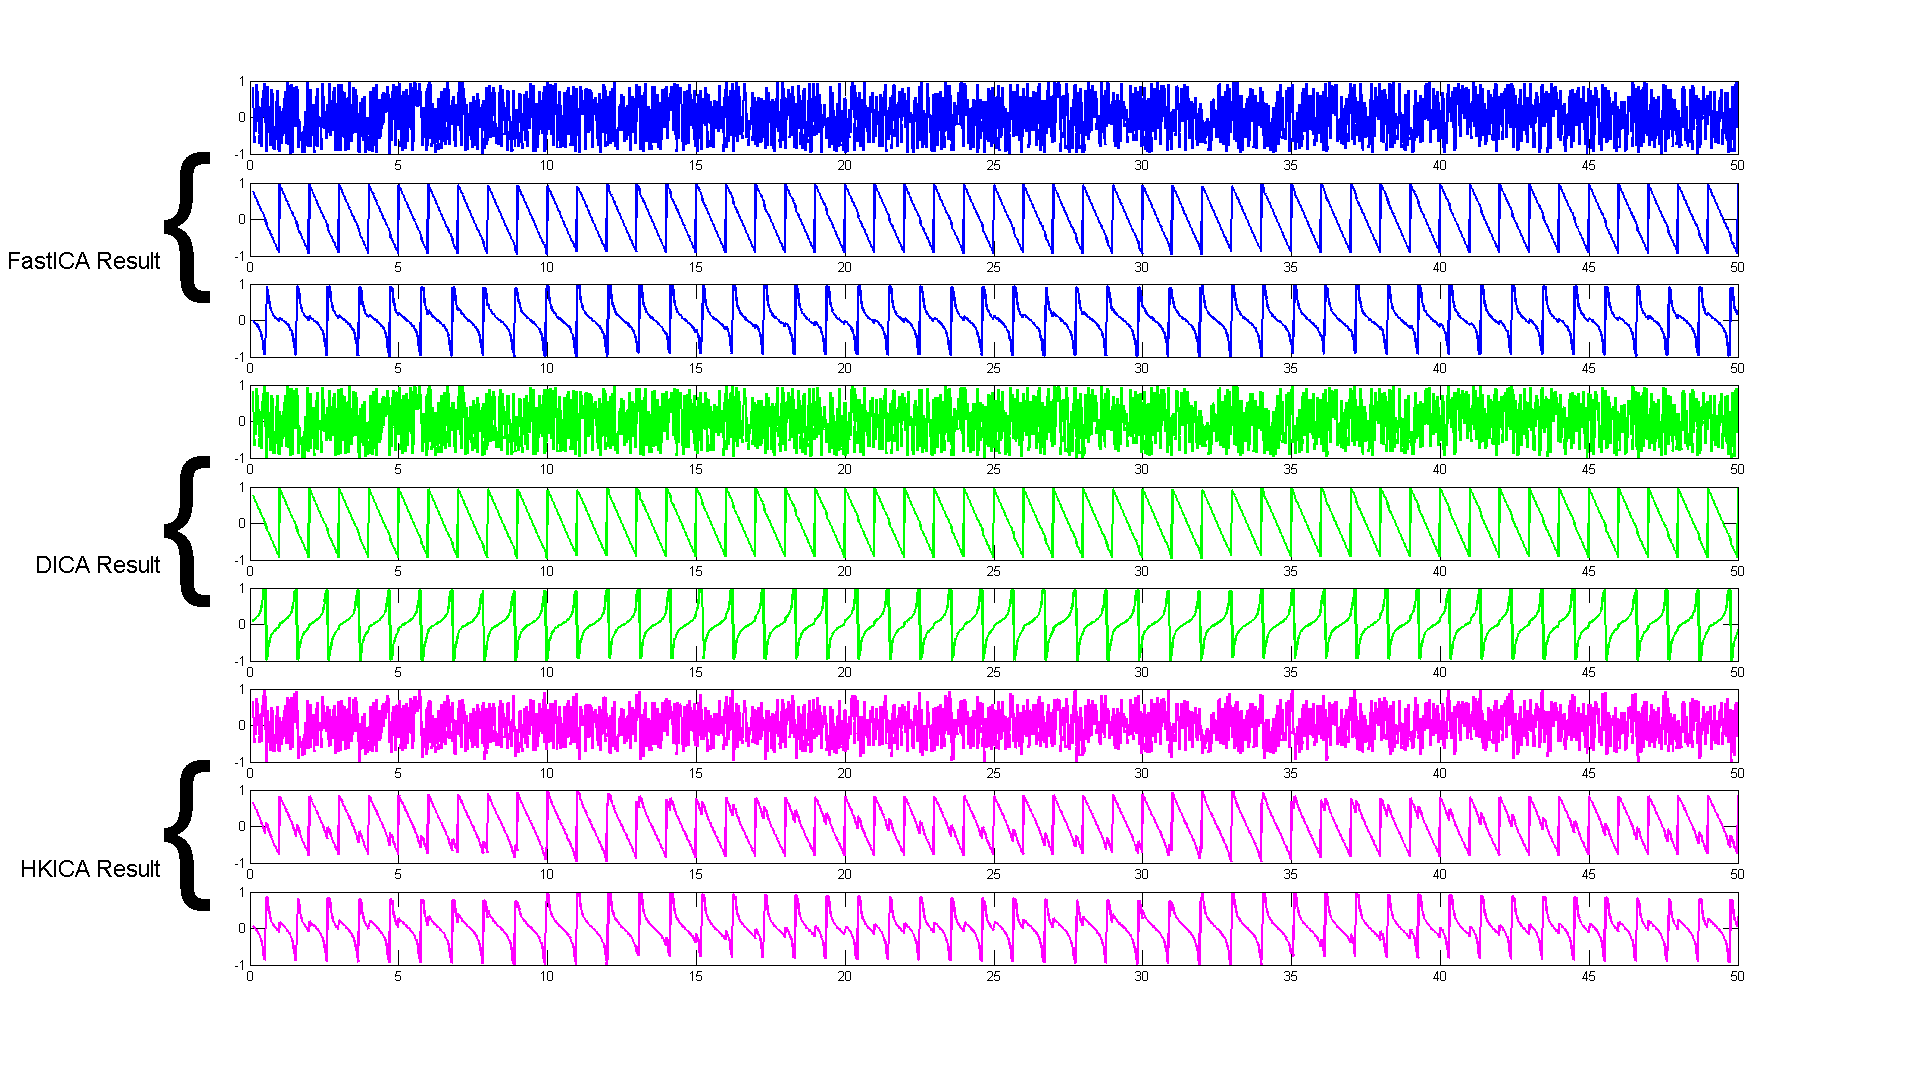
\includegraphics[width = 0.49\linewidth]{demo_res}
\caption{Example of ICA: The black signals are the source signals, red ones observed signals (left). The right figure shows the reconstructed (and rescaled) signals from FastICA, HKICA, and DICA (3 different ICA algorithms, see Section \ref{subsec:relatedWorks} and \ref{sec:DICA} for details ) after sampling $As(t)$ at 2500 uniformly spaced points in the interval $[0,50]$.}
\label{fig:demo}
\end{figure}

\if0
Independent Component Analysis (ICA)
%, as a main tool of blind source separation, 
has received much attention in the past decades. 
In the standard ICA model one can observe a $d$-dimensional vector $X$ that is a linear mixture of $d$ independent variables $(S_1,\ldots, S_d)$ with Gaussian noise:
\begin{equation}
\label{eq:stoch-ICA}
X = AS+\epsilon,
\end{equation}
where $\epsilon \sim \mathcal{N}(0,\Sigma)$ is a $d$-dimensional Gaussian noise with zero mean and covariance matrix $\Sigma$, and $A$ is a nonsingular $d \times d$ mixing matrix. 
The goal of the observer is to recover (separate) the source signals and the mixing matrix given several independent and identically distributed (\iid) observations from the above model based on the information on the independence only.
The ICA literature is vast in both practical algorithms and theoretical analyses; 
we refer to the book of \citet{comon2010handbook} for a comprehensive survey.
In practice, ICA is also known to work well for unmixing the mixture of various deterministic signals. 
One of the classical demonstrations of ICA is showing that two periodic signals can be well recovered from their mixtures \citep{HyvOja00}.
Such an example is shown in Figure~\ref{fig:demo}. 
This phenomenon suggests that the usual probabilistic notion is unsatisfactory if one wishes to have a deeper understanding of ICA.  

The main contribution of our paper is to analyze ICA algorithms in a deterministic framework. 
Our deterministic analysis helps investigate this curious phenomenon. Our result can be applied to more general setting without losing any generality to the traditional stochastic setting. 
Formally, instead of observing $T$ \iid samples from \eqref{eq:stoch-ICA}, the observations and the source signals are defined by the functions  $x:\natural \ra \real^d$ and $s:\natural \ra \real^d$ as $d$-dimensional deterministic functions. 
We study the question that to what extent can the mixture of signals be separated. 
We proposed a \emph{provable polynomial-time} algorithm that has \emph{no free parameter} for the noisy ICA model.
The analysis of the algorithm's performance is reduced to perturbation analysis, which depends on how much the observation function is deviated from the stochastic model. 
We proposed a data-dependent measure for such deviation based on the empirical distribution of data.
It can be shown that this measure converges to 0 in a rate of $O(\sqrt{T})$ for $T$ \iid samples from  \eqref{eq:stoch-ICA}.
Therefore when applied to the stochastic model, our algorithm is guaranteed to correctly reconstruct the mixing matrix $A$.

The rest of this paper is organized as follows: 
Our main results are highlighted in Section~\ref{sec:main}.
The polynomial-time algorithms underlying these results are developed through Section~\ref{sec:DICA}.
Due to space limit, proofs and experimental results are presented in the full version of the paper \citep{HuGySz15}.
\fi
 
\subsection{Notation}
We denote the set of real and natural numbers by $\real$ and $\natural$, respectively.
A vector $v \in K^d$ for a field $K$ is assumed to be a column vector.
The $2$-norm of $v$ is denoted by  $\|v\|_2$ and for any matrix $Z$ we let $\|Z\|_2=\max_{v:\|v\|_2=1}{\|Z v\|_2}$ denote the corresponding induced norm. 
%We denote the largest (smallest) singular value of $Z$ by $\sigma_{\max}(Z)$ (resp., by $\sigma_{\min}(Z)$). 
%Also, let $Z_{:i}$ denote the $i$th column of $Z$.
For a tensor (including vectors and matrices) $T$, its Frobenius norm (or $\ell_2$ norm) $\|T\|_F$  is defined as the square root of the sum of the square of all the entries.  
%For a vector $v=(v_1,\ldots,v_d) \in K^d$, $\vert v \vert$ is defined coordinatewise, that is $\vert v \vert=(\vert v_1 \vert,\ldots,\vert v_d\vert)$. 
The transpose of a vector/matrix $Z$ is denoted by $Z^\top$, while the inverse of the transpose is denoted by $Z^{-\top}$.  
The outer product of two vectors $v, u \in K^d$ is denoted by $u\otimes v=u v^\top$. 
Let $v^{\otimes k}$ denote the $k$-fold outer product of $v$ with itself, that is, $v\otimes v\otimes v \ldots \otimes v$, which is a k-dimensional tensor.
%Given a $4$-dimensional tensor $T$, we denote the matrix $Z$ by $T(\eta,\eta,\cdot , \cdot)$ that is generated by marginalizing the first two coordinates of $T$ on the direction $\eta$, that is,
%$Z_{i,j} = \sum_{k_1,k_2 = 1}^{d} \eta_{k_1} \eta_{k_2} T_{k_1,k_2,i,j}$. (Similar definitions for marginalizing different coordinates of the tensor.)
%For a real vector $v$ and some real number $C$, $v \le C$ means that all the entries of $v$ are at most $C$. 
%The bold symbol $\boldsymbol{1}$ denotes a vector with all entries being $1$ (the dimension of this vector will always be clear from the context).
Finally, $\poly{\cdot,\cdots,\cdot}$ denotes a polynomial function of its argument.

\section{Main Results}
\label{sec:main}
Let $x$, $s$, and $\epsilon$ be $\real^d$-valued functions from $[T]\doteq\{1,2,\ldots,T\}$, and $A$ be $d\times d$ nonsingular ``mixing'' matrix, such that 
\begin{equation}
\label{eq:ICA}
x(t) = As(t)+\epsilon(t), \qquad 1\le t\le T\,.
\end{equation}
We consider the problem of reconstructing $A$ having observed $x$ provided that $(A,s,\epsilon)$ are ``nice'' as it will be defined later. Intuitively, $s$ is the source whose components are ``independent'' while $\epsilon$ is ``noise''.
%Assume that we can observe the $d$ dimensional mixed signal $x(t) \in \real^d, t \in [T]:=\{1,2,\ldots,T\}$ generated by  
%Given observations  $x(t) \in \real^d, t \in [T]:=\{1,2,\ldots,T\}$, for any $d\times d$ nonsingular mixing matrix $A$, bounded $d$-dimensional function $s:[T] \to [-C,C]^d$, and $\epsilon:[T] \to \real^d$ such that
%where $A$ is a $d\times d$ nonsingular mixing matrix,  $s:[T] \to [-C,C]^d$ is a bounded, $d$-dimensional source function for some constant $C \ge 1$. , and $\epsilon:[T] \to \real^d$ is the noise function. 
We measure how well a matrix $\hat{A}$ returned by an algorithm working on data $x$ 
recovers $A$ by the reconstruction error defined as
\[
d(\hat{A}, A) = \inf_{
		\substack{\pi \in \mathrm{Perm}([d]) \\ c\in \real^d}} 
		\max_{k} || c_k A_{:\pi(k)} - A_{:k} ||_2\,,
\]
where $A_{:i}$ stands for the $i$th column of $A$ and
$\mathrm{Perm}([d])$ is the set of all the permutations on the set $[d]$.
This measure compensates for the inherent indeterminacy in reconstructing the scale and ordering of sources.

Let us now develop the ``niceness'' measure of the $(x,A,s,\eps)$. 
Starting from the classical setting, we will define this tuple nicer if the respective \emph{empirical} 
distributions approximately satisfy the usual assumptions: 
\begin{inparaenum}[\itshape a\upshape)]
\item the source ($s$) components are independent;
\item they have high absolute excess kurtosis;
\item they have zero mean;
\item the noise ($\eps$) has  zero mean;
\item it has low absolute excess kurtosis;
\item the noise and sources are independent.
\end{inparaenum}

%We will denote the $i$th component of $s$ by $s_i$. 
For a function $u:[T] \to \real^k$, we let $\nu^{(u)}$ stand for the empirical distribution of $u$,
defined by
$\nu^{(u)}(B)=\tfrac{1}{T}|\{t \in [T]: u(t) \in B\}|$ for Borel sets $B \subset \real^k$.
For a distribution $\mu$ over the reals we let $\kappa(\mu)$ be the (absolute excess) kurtosis of $\mu$: 
$\kappa(\mu) = |\int x^4 \mu(dx) - 3 (\int x^2 \mu(dx))^2|$.
For a product distribution $\mu= \mu_1\otimes \ldots \otimes \mu_d$ over $\real^d$, we let $\kappa_{\min}(\mu)
=\min_{1\le i \le d} \kappa(\mu_i)$ to denote the minimum kurtosis of the components of $\mu$.
When $\mu$ is a distribution over $\real^d$, we define the $d$-dimensional excess absolute kurtosis of $\mu$ by
$\kappa^2(\mu) = \max_{1\le i,j\le d} \sum_{k,l} 
\left\{ 
M_{i,j,k,l}(\mu)  - (M_{i,j}(\mu) M_{k,l}(\mu)+ 2 M_{i,k}(\mu) M_{j,l}(\mu))
\right\}^2$, where $M_{a,\dots,z}(\mu) = \int y_a \dots y_z \mu(dy)$.
We will also use $N(\nu) = \|\int x \nu(dx)\|$.

To measure the degree of independence of the components of the source $s$, we define
a family of ``distances'' to between distributions (strictly speaking, these are only pseudo-distances).
In particular, given two distributions $\nu_1$ and $\nu_2$ over $\real^d$ and an integer $k\ge 1$, we
let $D_k(\nu_1,\nu_2) = \sup_{f\in\mathcal{F}} |\int f(s)\nu_1(ds) - \int f(s)\nu_2(ds)|$, 
where $\mathcal{F}=\{f:\real^d \to \real : f(s)=\prod_{j=1}^k s_{i_j}, 1 \le i_1,\ldots,i_k \le d\}$ 
is the set of all monomials up to degree $k$.
When $\mu$ is a product measure, $D_k(\mu,\nu)$ measures how close the components of $X\sim \nu$ are to being independent.
%Also let $D_k(\nu)  = \inf_{\mu} D_k(\mu, \nu)$ where the infimum is taken over all the product measures.
%Hence, $D_k(\nu)$ measures how close is $\nu$ to be a product measure, i.e., $D_k(\nu)$ quantifies the degree of independence of the individual components of $X\sim \nu$.
When $\nu$ is a measure of $p+q$ variables (i.e., $X\in \real^{p+q}$) 
we also need a measure that quantifies the degree of independence of the vectors $(X_1,\dots,X_p)$ and $(X_{p+1},\dots,X_{p+q})$. We will denote this measure by $D_k^{(p,q)}(\nu)$ and is defined as $D_k^{(p,q)} (\nu)= \inf_{\mu_1,\mu_2} D_k(\mu_1\otimes \mu_2,\nu)$, where $\mu_1$ ranges over all measures on $\real^p$ and $\mu_2$ ranges over all measures on $\real^q$. 
Finally, we let 
\[
L = \max \left( \| \textstyle\int  [y^{\otimes 2}] \nu^{(\epsilon)}(dy) \|_F,\, 
			  \| \int  [y^{\otimes 3}] \nu^{(\epsilon)}(dy) \|_F \right),
\]
which captures the magnitude of second and third moments of the noise.
\if0
For any $p\ge 1$, $\eta\in \real^d$, and distribution $\nu$ over $\real^d$,
let 
$m_p^{(\nu)}(\eta) = \E_{X\sim \nu}[ (\eta^\top X)^p ],\, f_{\nu}(\eta) = \tfrac1{12} \left( m_4^{(\nu)}(\eta) - 3 m_2^{(\nu)}(\eta)^2 \right)$.
We also need to measure the perturbation of the second derivative of the function $f_{\nu_T^{(x)}}(\eta)$ caused by the noise function $\epsilon$, by 
\[
\mathcal{C}G(T) = \max_{\|\eta\|_2\le 1}\| \nabla^2f_{\nu_T^{(x)}}(\eta) - \nabla^2f_{\nu_T^{(As)}}(\eta) \|_2, 
\] 
for some problem dependent constant $\mathcal{C} = \poly{\sigma_{\max}, d, L}$. Note that $G(T)$ depends on how Gaussian $\epsilon$ is and how independent $\epsilon$ and $s$ are. 
In the standard stochastic setting, $G(T) = O(\frac{1}{\sqrt{T}})$.
\fi
%
\if0
We also need to measure how approximately $s$ and $\epsilon$ are 0 mean, how Gaussian the noise function $\epsilon$ is, and lastly how independent $s$ and $\epsilon$ are. Let 
\begin{align*}
G = &  \max \Huge{\{} \, \| \E_{S_i\sim \nu_T^{(s_i)}} [S_i] \|_F,\quad \| \E_{Y \sim \nu_T^{(\epsilon)}} [Y] \|_F, \\
& \quad  \max_{\|\eta\| \le 1} \Bigl\| \left(\E_{Y\sim \nu_T^{(\epsilon)}} [Y^{\otimes4}] - (\E_{Y\sim \nu_T^{(\epsilon)}} [Y^{\otimes2}])^{\otimes 2}\right)(\eta,\eta,\cdot,\cdot)  - 2 (\E_{Y\sim \nu_T^{(\epsilon)}} [Y^{\otimes2}])^{\otimes 2}(\eta,\cdot,\eta,\cdot)\Bigr\|_F, \\
& \quad \max_{
	\substack{i_1,i_2,j_1,j_2 \ge 0 \\ i_1+i_2+j_1+j_2 \le 4}}
 \| \E_{S\sim \nu_T^{(s)}} [(AS)^{\otimes i_1}\!\otimes \E_{Y\sim \nu_T^{(\epsilon)}} [Y^{\otimes j_1}] \!\otimes (AS)^{\otimes i_2}] \\
& \quad \quad \quad \quad - \E_{(S, Y)\sim \nu_T^{(s, \epsilon)}} [(AS)^{\otimes i_1}\!\otimes Y^{\otimes j_1}\!\otimes (AS)^{\otimes i_2}]  \|_F, \\
& \quad \max_{
	\substack{i_1,i_2,j_1,j_2 \ge 0 \\ i_1+i_2+j_1+j_2 \le 4}}
\| \E_{Y\sim \nu_T^{(\epsilon)}} [Y^{\otimes j_1} \otimes \E_{S\sim \nu_T^{(s)}} [(AS)^{\otimes i_1}] \otimes Y^{\otimes j_2}] \\
& \quad \quad \quad \quad - \E_{(S, Y)\sim \nu_T^{(s, \epsilon)}} [ Y^{\otimes j_1}\otimes (AS)^{\otimes i_1}\otimes Y^{\otimes j_2}] \|_F \, \Huge{\}}.
\end{align*}
\fi
We let $\Pi_0$ to be the set of zero mean product distributions over $\real^d$.

Now we are ready to state our main result. 
\begin{thm}
\label{thm:finalRes} 
There exists a randomized algorithm such that 
for any $A\in \real^{d\times d}$, and $x, s, \epsilon: [T] \rightarrow \real^d$ satisfying Equation \eqref{eq:ICA},
the algorithm returns $\hat{A}$
%Consider the ICA problem \eqref{eq:ICA}. There exists an algorithm that estimates the mixing matrix $A$ from $T$ samples of $x$ 
such that with probability at least $1-\delta$,
\[
d(\hat{A}, A) \le
\inf_{\mu\in \Pi_0} \mathcal{C}(\mu) \min\left(D_4(\nu^{(s)},\mu)+ \kappa(\nu^{(\eps)}) + D_4^{(d,d)}(\nu^{(As,\eps)})
+N(\nu^{(\eps)}) + N( \nu^{(s)}), \Theta(\mu) \right),
\]
where $\mathcal{C}(\mu)$ and $\Theta(\mu)$ are problem dependent constants, polynomial in $(\sigma_{\max}(A), 1/\sigma_{\min}(A), 1/\kappa_{\min}(\mu),1/\delta, d, L)$.
Further, the computational complexity of the algorithm is $O(d^3 T)$ when used on any data $x$ of dimensions $T\times d$.

\if0
if $S$ has distribution $\mu$ and
\[
T \ge \poly{d, \frac{1}{\kappa_{\min}}, \frac{1}{\delta}, C, \sigma_{\max}, \frac{1}{\sigma_{\min}}, \|\Sigma\|_2},
\]
then, with probability at least $1-\delta$, there exists a permutation $\pi$ and constants $\{c_1,\ldots,c_d\}$, such that for all $1\le k\le d$,
\begin{align*}
 \| c_k\hat{A}_{\pi(k)} - A_k\|_2 \le 
& \frac{\poly{C, \sigma_{\max}, \frac{1}{\sigma_{\min}}, \frac{1}{\kappa_{\min}},\frac{1}{\delta}, d}}{\sqrt{2T}}.
\end{align*}
\fi
\end{thm}
Note that the above result implies that in the standard stochastic setting
with independent sources and Gaussian noise, independently generated from the sources, 
with probability at least $1-\delta$,
\[
d(\hat{A}, A) \le \mathcal{C} \min\left(\tfrac{1}{\sqrt{T}}, \Theta \right),
\]
for some problem dependent constants $\mathcal{C}$ and $\Theta$.
The next section describes the algorithm that achieves this bound.
\if0
\subsection{Assumptions about the data}
\label{subsec:assumptions}
\begin{assumption}
\label{ass:gauss}
Assume there exists a constant $L$ and a function $g:\natural\rightarrow \real$ such that $g(t) \to 0$ as $t \to \infty$ and
\begin{enumerate}[(i)]
\item $\| \E_{S_i\sim \nu_t^{(s_i)}} [S_i] \|_F,\, \| \E_{Y \sim \nu_t^{(\epsilon)}} [Y] \|_F \le g(t)$; $\| \E_{Y\sim \nu_t^{(\epsilon)}} [Y^{\otimes 2}] \|_F,\, \| \E_{Y\sim \nu_t^{(\epsilon)}} [Y^{\otimes 3}] \|_F \le L$;
\item $\Bigl\| \left(\E_{Y\sim \nu_t^{(\epsilon)}} [Y^{\otimes4}] - (\E_{Y\sim \nu_t^{(\epsilon)}} [Y^{\otimes2}])^{\otimes 2}\right)(\eta,\eta,\cdot,\cdot)  - 2 (\E_{Y\sim \nu_t^{(\epsilon)}} [Y^{\otimes2}])^{\otimes 2}(\eta,\cdot,\eta,\cdot)\Bigr\|_F\le g(t)\|\eta\|_2^2$.
\end{enumerate}
Here $L$ and the function $g$ may depend on $\{A,\Sigma,C,d\}$.
\end{assumption}
\begin{assumption}
\label{ass:independence}
Assume the source signal function and the noise function are `independent' up to the 4th moment in the sense that for any $i_1,i_2,j_1,j_2 \ge 0$ such that $i_1+i_2+j_1+j_2 \le 4$,  
\[
 \| \E_{S\sim \nu_t^{(s)}} [(AS)^{\otimes i_1}\!\otimes \E_{Y\sim \nu_t^{(\epsilon)}} [Y^{\otimes j_1}] \!\otimes (AS)^{\otimes i_2}]
- \E_{(S, Y)\sim \nu_t^{(s, \epsilon)}} [(AS)^{\otimes i_1}\!\otimes Y^{\otimes j_1}\!\otimes (AS)^{\otimes i_2}]  \|_F 
 \le g(t),
\]
\[
\| \E_{Y\sim \nu_t^{(\epsilon)}} [Y^{\otimes j_1} \otimes \E_{S\sim \nu_t^{(s)}} [(AS)^{\otimes i_1}] \otimes Y^{\otimes j_2}]- \E_{(S, Y)\sim \nu_t^{(s, \epsilon)}} [ Y^{\otimes j_1}\otimes (AS)^{\otimes i_1}\otimes Y^{\otimes j_2}] \|_F 
\le g(t), % \le L/\sqrt{t},
\]
for the same function $g$ in Assumption \ref{ass:gauss}, where $(s,\epsilon)$ is the function obtained by concatenating $s$ and $\epsilon$ together.  
\end{assumption}
\begin{remark}
Assumption \ref{ass:gauss} (i) forces that the average of $s$ and $\epsilon$ decay to 0 at a rate of $g(t)$,
and that both the second and third moments of the noise be bounded.
Assumption \ref{ass:gauss} (ii) basically says that the induced measure of the noise function $\epsilon$ has 0 kurtosis in the limit.
Assumption \ref{ass:independence} is to guarantee that the source signals and the noise be approximately independent.
\end{remark}
\fi
\section{A Deterministic ICA Algorithm}
\label{sec:DICA}
The algorithm is inspired by \citet{hsu2013learning}, \citet{arora2012provable}, and \citet{frieze1996learning} using a quasi-whitening procedure:
%For any $p\ge 1$, $\eta\in \real^d$, and distribution $\nu$ over $\real^d$,
%let 
%$m_p^{(\nu)}(\eta) = \E_{X\sim \nu}[ (\eta^\top X)^p ],\, f_{\nu}(\eta) = \tfrac1{12} \left( m_4^{(\nu)}(\eta) - 3 m_2^{(\nu)}(\eta)^2 \right)$.
One can show that $\nabla^2 f_\mu(\psi)=A K D_{\psi} A^\top$ for any product measure $\mu$ where $D_{\psi} =\text{diag}\left((\psi^{\top}A_1)^2,\cdots, (\psi^{\top}A_d)^2\right)$,
and so $B= AK^{1/2}D_{\psi}^{1/2}R^{\top}$ for some orthonormal matrix $R$. Defining $T_i=\nabla^2 f_\mu(B^{-\top} \phi_i)$, one can calculate that
$T_i=A K^{1/2} D_\psi^{-1/2} \Lambda_i A^\top$ where $\Lambda_i =\text{diag}\left( (\phi_i^\top R_1)^2,\ldots,(\phi_i^\top R_d)^2 \right)$ and $R_i$ denote the $i$th column of $R$.
Then $M=T_1 T_2^{-1} = A\Lambda A^{-1}$ with $\Lambda=\Lambda_1 \Lambda_2^{-1}=\text{diag}\left( \left(\frac{\phi_1^\top R_1}{\phi_2^\top R_1}\right)^2,\ldots,\left(\frac{\phi_1^\top R_d}{\phi_2^\top R_d}\right)^2 \right)$. Thus, $A_i$ are again the eigenvectors of $M$.
Note that the eigenvalues of $M$ are defined in terms of the orthogonal matrix $R$,
and so it is easy to handle the resulting minimum spacing
\begin{equation}
\label{def:gammaR}
\gamma_R =  \min_{i,j: i\neq j} \left\vert \left(\frac{\phi_1^{\top}R_i}{\phi_2^{\top}R_i}\right)^2 - \left(\frac{\phi_1^{\top}R_j}{\phi_2^{\top}R_j}\right)^2 \right\vert.
\end{equation}
We show in the full version \citep{HuGySz15} %Lemma~\ref{lem:ConstantProb} in the appendix 
that, among others,  $\gamma_R \ge\frac{\delta}{2d^2}$ with probability at least $1-\delta$.
The resulting algorithm, called Deterministic ICA (DICA), is shown in Algorithm \ref{alg:DICA}. 
\begin{algorithm}
\caption{Deterministic ICA (DICA)}
\label{alg:DICA}
\begin{algorithmic}[1]
\INPUT $x(t)$ for $1\le t \le T$. 
\OUTPUT An estimation of the mixing matrix $A$. 
\STATE Sample $\psi$ from a $d$-dimensional standard Gaussian distribution;
\STATE Evaluate $\nabla^2\hat{f}(\psi)$, \\
%\quad where $\hat{m_p}(\eta) = \frac{1}{T}\sum_{k=1}^{T} (\eta^{\top}g(k))^p$, and $\hat{f}(\eta) = \frac{1}{12}\big(\hat{m_4}(\eta) - 3\hat{m_2}(\eta)^2 \big)$;
\STATE Compute $\hat{B}$ such that $\nabla^2\hat{f}(\psi) = \hat{B}\hat{B}^{\top}$;
\STATE Sample $\phi_1$ and $\phi_2$ independently from the standard Gaussian distribution;
\STATE Compute $\hat{T}_1 =\nabla^2\hat{f}(\hat{B}^{-\top}\phi_1)$ and  $\hat{T}_2 =\nabla^2\hat{f}(\hat{B}^{-\top}\phi_2)$;

\STATE Compute all the eigenvectors of $\hat{M} = \hat{T}_1\left(\hat{T}_2\right)^{-1}$, $\{\mu_1,\ldots,\mu_d\}$;
\STATE Return $\hat{A} = \{\mu_1,\ldots,\mu_d\}$.
\end{algorithmic}
\end{algorithm}

\subsection{Related Works}
\label{subsec:relatedWorks}
Perhaps the most popular approach to the ICA problem is the FastICA algorithm \citep{hyvarinen1999fast}. 
Great progress has been made to analyze FastICA theoretically \citep{tichavsky2006performance,oja2006fastica,ollila2010deflation,dermoune2013fastica,wei2014convergence}.
In particular, recently \citet{miettinen2014fourth} showed that in the noise-free case (i.e., when $X = AS$), the error of FastICA (when using a particular forth-moments-based contrast function) vanishes at a rate of $1/\sqrt{T}$ where $T$ is the sample size.
In addition, several other methods have been shown to achieve similar error rates in the noise-free setting \citep[e.g.,][]{eriksson2003characteristic,samarov2004nonparametric,chen2005consistent,chen2006efficient}.
However, to our knowledge, no similar finite sample results are available in the noisy case.

On the other hand, promising algorithms based on moment methods are available in the noisy case that make significant advances towards provably efficient and effective ICA algorithms, albeit fall short of either providing a complete solution or providing rigorous proofs. \citep{anandkumar2012tensordecomposition,anandkumar2012method, arora2012provable, hsu2013learning, goyal2014fourier}
In particular, the results of \citep{arora2012provable} and \cite{goyal2014fourier} depend on some  unspecified parameters ($\beta$ in the paper of \citep{arora2012provable} and $\sigma$ in the paper of \citep{goyal2014fourier}) that are belong some specific range, making their algorithms impossible to tune.
A common problem faced by the other methods (\citep{anandkumar2012tensordecomposition,anandkumar2012method,hsu2013learning}) is a minimal gap of the eigenvalues, which may result in an exponential dependence on the number of source signals $d$. 
Recently, \citet{vempala2014max} proposed an ICA algorithm based on an elegant, recursive version of the method of \citet{goyal2014fourier} that avoids dealing with the aforementioned minimal gap; however, they still need an oracle to set the unspecified parameter of \citet{goyal2014fourier}.

The problem of separating mixture of deterministic signals are also consider in \citep{kirimoto2011separation} and \citep{forootan2013separation}. But the analysis is restricted to particular signals, while our result is applicable to general ones.

\subsubsection*{Acknowledgments}
This work was supported by the Alberta Innovates Technology Futures and NSERC.
\bibliographystyle{plainnat}
\bibliography{DICA}
\end{document}
